% Options for packages loaded elsewhere
\PassOptionsToPackage{unicode}{hyperref}
\PassOptionsToPackage{hyphens}{url}
\PassOptionsToPackage{dvipsnames,svgnames,x11names}{xcolor}
%
\documentclass[
]{article}

\usepackage{amsmath,amssymb}
\usepackage{setspace}
\usepackage{iftex}
\ifPDFTeX
  \usepackage[T1]{fontenc}
  \usepackage[utf8]{inputenc}
  \usepackage{textcomp} % provide euro and other symbols
\else % if luatex or xetex
  \usepackage{unicode-math}
  \defaultfontfeatures{Scale=MatchLowercase}
  \defaultfontfeatures[\rmfamily]{Ligatures=TeX,Scale=1}
\fi
\usepackage{lmodern}
\ifPDFTeX\else  
    % xetex/luatex font selection
\fi
% Use upquote if available, for straight quotes in verbatim environments
\IfFileExists{upquote.sty}{\usepackage{upquote}}{}
\IfFileExists{microtype.sty}{% use microtype if available
  \usepackage[]{microtype}
  \UseMicrotypeSet[protrusion]{basicmath} % disable protrusion for tt fonts
}{}
\makeatletter
\@ifundefined{KOMAClassName}{% if non-KOMA class
  \IfFileExists{parskip.sty}{%
    \usepackage{parskip}
  }{% else
    \setlength{\parindent}{0pt}
    \setlength{\parskip}{6pt plus 2pt minus 1pt}}
}{% if KOMA class
  \KOMAoptions{parskip=half}}
\makeatother
\usepackage{xcolor}
\setlength{\emergencystretch}{3em} % prevent overfull lines
\setcounter{secnumdepth}{5}
% Make \paragraph and \subparagraph free-standing
\makeatletter
\ifx\paragraph\undefined\else
  \let\oldparagraph\paragraph
  \renewcommand{\paragraph}{
    \@ifstar
      \xxxParagraphStar
      \xxxParagraphNoStar
  }
  \newcommand{\xxxParagraphStar}[1]{\oldparagraph*{#1}\mbox{}}
  \newcommand{\xxxParagraphNoStar}[1]{\oldparagraph{#1}\mbox{}}
\fi
\ifx\subparagraph\undefined\else
  \let\oldsubparagraph\subparagraph
  \renewcommand{\subparagraph}{
    \@ifstar
      \xxxSubParagraphStar
      \xxxSubParagraphNoStar
  }
  \newcommand{\xxxSubParagraphStar}[1]{\oldsubparagraph*{#1}\mbox{}}
  \newcommand{\xxxSubParagraphNoStar}[1]{\oldsubparagraph{#1}\mbox{}}
\fi
\makeatother


\providecommand{\tightlist}{%
  \setlength{\itemsep}{0pt}\setlength{\parskip}{0pt}}\usepackage{longtable,booktabs,array}
\usepackage{calc} % for calculating minipage widths
% Correct order of tables after \paragraph or \subparagraph
\usepackage{etoolbox}
\makeatletter
\patchcmd\longtable{\par}{\if@noskipsec\mbox{}\fi\par}{}{}
\makeatother
% Allow footnotes in longtable head/foot
\IfFileExists{footnotehyper.sty}{\usepackage{footnotehyper}}{\usepackage{footnote}}
\makesavenoteenv{longtable}
\usepackage{graphicx}
\makeatletter
\newsavebox\pandoc@box
\newcommand*\pandocbounded[1]{% scales image to fit in text height/width
  \sbox\pandoc@box{#1}%
  \Gscale@div\@tempa{\textheight}{\dimexpr\ht\pandoc@box+\dp\pandoc@box\relax}%
  \Gscale@div\@tempb{\linewidth}{\wd\pandoc@box}%
  \ifdim\@tempb\p@<\@tempa\p@\let\@tempa\@tempb\fi% select the smaller of both
  \ifdim\@tempa\p@<\p@\scalebox{\@tempa}{\usebox\pandoc@box}%
  \else\usebox{\pandoc@box}%
  \fi%
}
% Set default figure placement to htbp
\def\fps@figure{htbp}
\makeatother
% definitions for citeproc citations
\NewDocumentCommand\citeproctext{}{}
\NewDocumentCommand\citeproc{mm}{%
  \begingroup\def\citeproctext{#2}\cite{#1}\endgroup}
\makeatletter
 % allow citations to break across lines
 \let\@cite@ofmt\@firstofone
 % avoid brackets around text for \cite:
 \def\@biblabel#1{}
 \def\@cite#1#2{{#1\if@tempswa , #2\fi}}
\makeatother
\newlength{\cslhangindent}
\setlength{\cslhangindent}{1.5em}
\newlength{\csllabelwidth}
\setlength{\csllabelwidth}{3em}
\newenvironment{CSLReferences}[2] % #1 hanging-indent, #2 entry-spacing
 {\begin{list}{}{%
  \setlength{\itemindent}{0pt}
  \setlength{\leftmargin}{0pt}
  \setlength{\parsep}{0pt}
  % turn on hanging indent if param 1 is 1
  \ifodd #1
   \setlength{\leftmargin}{\cslhangindent}
   \setlength{\itemindent}{-1\cslhangindent}
  \fi
  % set entry spacing
  \setlength{\itemsep}{#2\baselineskip}}}
 {\end{list}}
\usepackage{calc}
\newcommand{\CSLBlock}[1]{\hfill\break\parbox[t]{\linewidth}{\strut\ignorespaces#1\strut}}
\newcommand{\CSLLeftMargin}[1]{\parbox[t]{\csllabelwidth}{\strut#1\strut}}
\newcommand{\CSLRightInline}[1]{\parbox[t]{\linewidth - \csllabelwidth}{\strut#1\strut}}
\newcommand{\CSLIndent}[1]{\hspace{\cslhangindent}#1}

\usepackage{titling}
\usepackage[noblocks]{authblk}
\renewcommand*{\Authsep}{, }
\renewcommand*{\Authand}{, }
\renewcommand*{\Authands}{, }
\renewcommand\Affilfont{\small}
\makeatletter
\@ifpackageloaded{caption}{}{\usepackage{caption}}
\AtBeginDocument{%
\ifdefined\contentsname
  \renewcommand*\contentsname{Table of contents}
\else
  \newcommand\contentsname{Table of contents}
\fi
\ifdefined\listfigurename
  \renewcommand*\listfigurename{List of Figures}
\else
  \newcommand\listfigurename{List of Figures}
\fi
\ifdefined\listtablename
  \renewcommand*\listtablename{List of Tables}
\else
  \newcommand\listtablename{List of Tables}
\fi
\ifdefined\figurename
  \renewcommand*\figurename{Figure}
\else
  \newcommand\figurename{Figure}
\fi
\ifdefined\tablename
  \renewcommand*\tablename{Table}
\else
  \newcommand\tablename{Table}
\fi
}
\@ifpackageloaded{float}{}{\usepackage{float}}
\floatstyle{ruled}
\@ifundefined{c@chapter}{\newfloat{codelisting}{h}{lop}}{\newfloat{codelisting}{h}{lop}[chapter]}
\floatname{codelisting}{Listing}
\newcommand*\listoflistings{\listof{codelisting}{List of Listings}}
\makeatother
\makeatletter
\makeatother
\makeatletter
\@ifpackageloaded{caption}{}{\usepackage{caption}}
\@ifpackageloaded{subcaption}{}{\usepackage{subcaption}}
\makeatother

\usepackage{bookmark}

\IfFileExists{xurl.sty}{\usepackage{xurl}}{} % add URL line breaks if available
\urlstyle{same} % disable monospaced font for URLs
\hypersetup{
  pdftitle={Policy Analysis on Incorporating A.I. into Academic Institutions for Research Commercialization},
  pdfauthor={Matthew Lyn},
  colorlinks=true,
  linkcolor={blue},
  filecolor={Maroon},
  citecolor={Blue},
  urlcolor={Blue},
  pdfcreator={LaTeX via pandoc}}



\title{Policy Analysis on Incorporating A.I. into Academic Institutions
for Research Commercialization\\[2.0ex]\large M.S. Biotechnology Program
- Spring 2025}

\author[1]{Matthew Lyn}
\author[2]{Christon Hill}

\affil[1]{Georgetown University - Department of Biochemistry \&
Molecular \& Cellular Biology 3900 Reservoir Rd NW, Washington D.C.
20057}
\affil[2]{Georgetown University - Office of Technology
Commercialization 2115 Wisconsin Avenue, NW, Suite G202, Washington D.C.
20007}

\date{}
\begin{document}
\maketitle

\renewcommand*\contentsname{Table of contents}
{
\hypersetup{linkcolor=}
\setcounter{tocdepth}{3}
\tableofcontents
}

\setstretch{1.15}
\section{Abstract}\label{abstract}

This research project, undertaken on behalf of the Georgetown University
Office of Technology Commercialization (OTC), analyzed both 1) scholarly
literature on the adoption of Artificial Intelligence (AI) into academic
institutions and 2) an organizationally circulated survey assessing
preconceptions of AI, and the complexity of tasks for which AI could be
productively applied. Finally, this project offers several policy
recommendations for the safe, sustainable, and productive use of
Artificial Intelligence (AI) in the commercialization of academic
research.

\section{Introduction}\label{sec-intro}

This project specifically examines the policy issues present at the
intersection of academic institutions and the technology
commercialization offices which assists researchers in creating
contractually licensable/purchasable Intellectual Property (IP) from
academic research. The creation of, and adherence to policies governing
the safe and effective usage of AI in biotechnology is a matter of
increasing international importance: the U.S. Senate's National
Commission on Emerging Biotechnology suggests a \emph{minimum}
investment by Congress of \$15 billion dollars over five years,
specifically targeting the intersection of biology and AI (Young et al.
2025).

However, without policy guidance or a method of measuring compliance,
the regulatory, economic, and public-facing risks multiply, rather than
decrease ((PWC) Price Waterhouse Coopers n.d.). Higher Education (HE)
institutions (like Georgetown itself ({``Initiative on Pedagogical Uses
of Artificial Intelligence. Georgetown University - Center for New
Designs in Learning \& Scholarship''} n.d.)) and publishing
organizations (like Nature ({``Artificial Intelligence ({AI}) {\textbar}
Nature Portfolio Editorial Policies''} n.d.)), have generally delegated
authority to the individual level. Thus, the discourse on effective AI
policy at these key intersections has been largely unexplored.

\subsection{Objective}\label{objective}

This research project seeks to analyze scholarly literature and a
organizationally circulated survey to investigate critical contemporary
barriers, uncertainties, and deficits in policy guidance for the safe,
sustainable, and productive use of Artificial Intelligence (AI) in
research commercialization, before offering several policy
recommendations.

\section{Methods \& Materials}\label{methods-materials}

\subsection{Literature Review}\label{literature-review}

Scholarly articles on the current state of organizational policy on the
safe, effective, and productive use of AI at the intersection of
biotechnology and higher education was collected via the Georgetown
University Dahlgren Memorial Library online services. Articles were
selected based on their relevance for literature review before being
sorted into three major categories: 1. Current Policy Guidance 2.
Adoption of AI in Biotechnology Research 3. Risk, Safety, and Compliance
Policy on AI.

A preliminary review screened these articles for inclusion or removal,
with specific emphasis on including 1) AI-related articles submitted
with corporate co-authors for their proximity and insight into the
design, creation, and improvement of generative AI models, 2) Policy
papers submitted by congressional, think-tank, and/or university
departments for their respective proximity to the issues outlined in
Section2, and 3) management consulting companies with ``well-regarded''
risk, safety, and compliance practices.

\subsection{Organizational Survey:}\label{organizational-survey}

An organizational survey (n=6) was circulated among stakeholders at the
Georgetown University - Office of Technology Commercialization to assess
existing attitudes on generative AI, as well as the existing office
tasks best-suited for AI automation. Survey answer format was a modified
Likert Scale (Joshi et al. 2015), while survey question format for task
complexity was formulated using a modified NASA Task Load Index
(Hoonakker et al. 2011), and AI attitudes using Net Promoter Score
({``Net Promoter Score ({NPS}): The Ultimate Guide. Qualtrics''} n.d.).

\section{Methods \& Materials}\label{methods-materials-1}

\subsection{Literature Review}\label{literature-review-1}

Scholarly articles on the current state of organizational policy on the
safe, effective, and productive use of AI at the intersection of
biotechnology and higher education was collected via the Georgetown
University Dahlgren Memorial Library online services. Articles were
selected based on their relevance for literature review before being
sorted into three major categories:

\begin{enumerate}
\def\labelenumi{\arabic{enumi}.}
\tightlist
\item
  Current Policy Guidance
\item
  Adoption of AI in Biotechnology Research
\item
  Risk, Safety, and Compliance Policy on AI
\end{enumerate}

A preliminary review screened these articles for inclusion or removal,
with specific emphasis on including 1) AI-related articles submitted
with corporate co-authors for their proximity and insight into the
design, creation, and improvement of generative AI models, 2) Policy
papers submitted by congressional, think-tank, and/or university
departments for their respective proximity to the issues outlined in
Section~\ref{sec-intro}, and 3) management consulting companies with
``well-regarded'' risk, safety, and compliance practices.

\subsection{Organizational Survey}\label{organizational-survey-1}

An organizational survey (n=6) was circulated among stakeholders at the
Georgetown University - Office of Technology Commercialization to assess
existing attitudes on generative AI, as well as the existing office
tasks best-suited for AI automation. Survey answer format was a modified
Likert Scale (Joshi et al. 2015), while survey question format for task
complexity was formulated using a modified NASA Task Load Index
(Hoonakker et al. 2011), and AI attitudes using Net Promoter Score
({``Net Promoter Score ({NPS}): The Ultimate Guide. Qualtrics''} n.d.).

\section{Results \& Conclusion}\label{results-conclusion}

\subsection{Significance}\label{significance}

The application of AI in research commercialization would 1)
definitively align with numerous legislative activities for
fast-tracking the transmutation of biotech research into economic value,
and 2) follow the widespread adoption of AI in biotechnology research in
general (Kim et al. 2025). AI's ability to form miniature ``literature
review committees'' within multi-agent LLM paradigms has led to
significant productivity improvements in AI's capability as a
``co-scientist'': identifying both the genes responsible for; and
formulating organic compounds for effectively mitigating; anti-microbial
resistance in bacteria (Gottweis et al. 2025), (Penadés et al. 2025).

But these gains in AI's information synthesis and reasoning capabilities
are yet to be proportionately applied in business domains as they have
been in biotechnology research (Kim et al. 2025), representing a key
bottle-neck (or ``knowledge filter'' (Acs et al. 2012)) in translating
publicly funded research into economic value creation (Aldridge and
Audretsch 2011). The application of AI in research commercialization
offices is well suited given the density of expert-level, domain
specific information vital to the successful transition of research into
economically viable and publicly accessible IP.

\subsection{\texorpdfstring{Literature Review:
Figure~\ref{fig-r-meta-review}}{Literature Review: Figure~}}\label{sec-r-lit-review}

\begin{figure}

\centering{

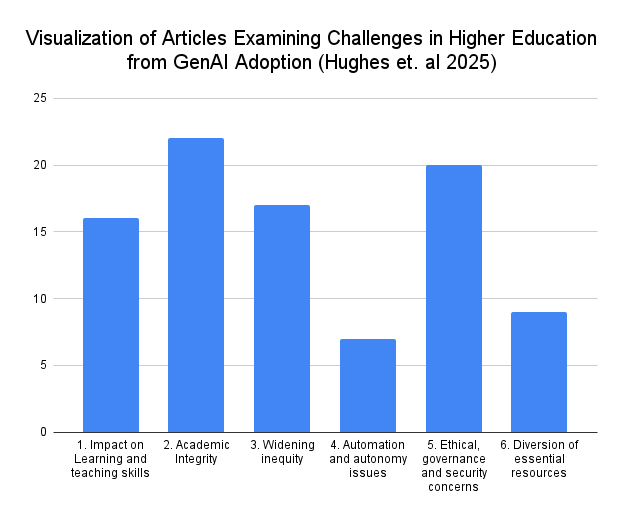
\includegraphics[width=5in,height=\textheight,keepaspectratio]{images/meta_review.png}

}

\caption{\label{fig-r-meta-review}A meta-review by (Hughes et al. 2025)
collected a variety of sources discussing the impact of Generative AI on
Higher Education. The visualization counting the number of sources by
topic was created by the author.}

\end{figure}%

Examining Figure~\ref{fig-r-meta-review}, the most popularly discussed
policy topics in (Hughes et al. 2025) meta-review are listed for (n=49)
sources with potential overlap for each source. From
Figure~\ref{fig-r-meta-review}, the ranked order of key topics is 1)
Academic Integrity, 2) Ethical, Governance, and Security Concerns, and
3) Widening Inequity.

\textbf{Academic Integrity} was the most frequently cited concern,
reflecting ongoing debates over proper attribution of AI‑generated
contributions, preservation of originality in patentable inventions, and
verifiable validity/source of research data---each directly affecting
downstream intellectual‑property negotiations.

\textbf{Ethical, Governance, and Security} considerations form the
second‑largest cluster; comprising the risks related to data privacy,
which is specifically relevant in this context given the variety of
confidential/controlled information prioritized for IP protection,
emphasizing the need for governance structures and audit mechanisms
before AI are cleared for handling sensitive documents (Gupta et al.
2023).

Finally, the theme of \textbf{Widening Inequity}, though comparatively
less prominent, examines whether uneven access to computational
resources and proprietary training data may compound existing
disparities between well‑funded and resource‑constrained universities,
thereby shaping which discoveries ultimately reach the marketplace.

Collectively, these three topics provide a limited policy-agenda for
technology‑transfer offices seeking to safeguard research integrity,
manage risk, and promote equitable value creation.

\subsection{\texorpdfstring{Organizational Survey: Figure~\ref{fig-r-ai}
\&
Figure~\ref{fig-r-task}}{Organizational Survey: Figure~ \& Figure~}}\label{sec-r-org-survey}

\begin{figure}

\centering{

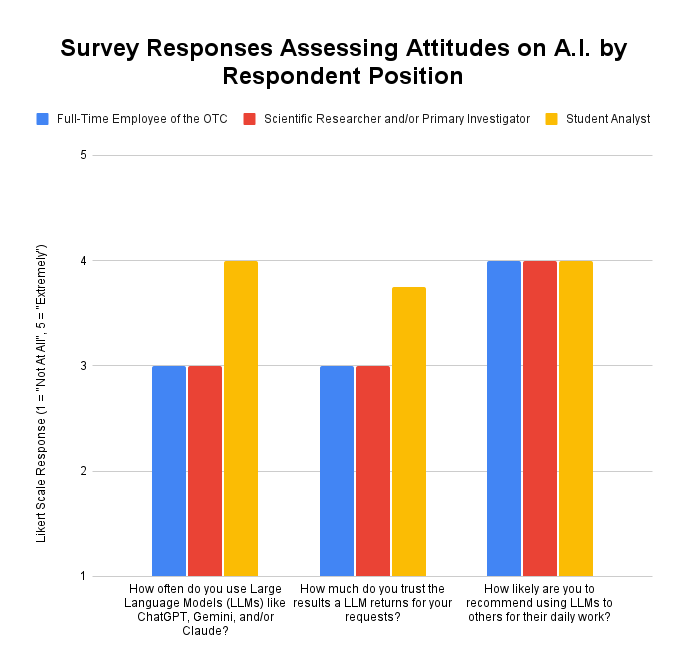
\includegraphics[width=6in,height=\textheight,keepaspectratio]{images/ai_position.png}

}

\caption{\label{fig-r-ai}Survey Responses measuring attitudes on
Generative AI using Modifed 1-5 Likert Scale.}

\end{figure}%

\begin{figure}

\centering{

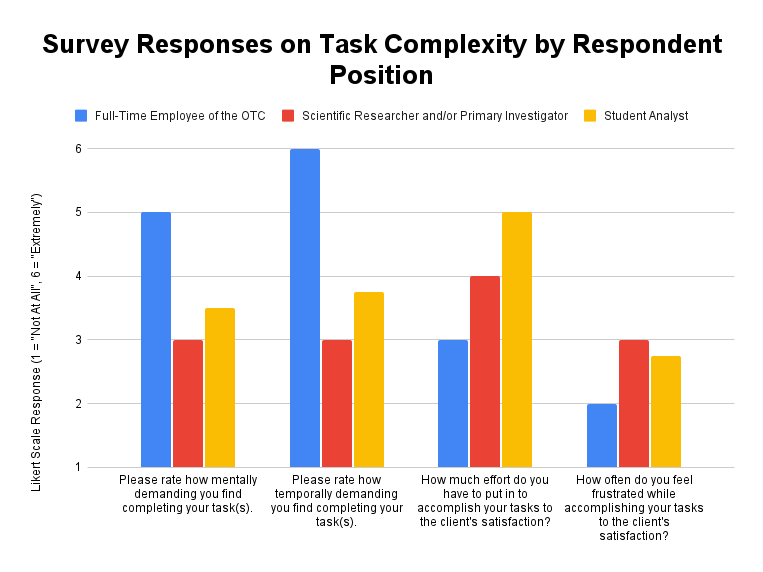
\includegraphics[width=6in,height=\textheight,keepaspectratio]{images/task_position.png}

}

\caption{\label{fig-r-task}Survey responses on the self-reported demand
of the tasks assigned to their job-title. These questions were
formulated using the NASA Task Load Index quantification strategy
(Hoonakker et al. 2011) on a modified 1-6 Likert Scale.}

\end{figure}%

Examining Figure~\ref{fig-r-ai} \& Figure~\ref{fig-r-task}, there
appears to be a general, positive disposition of student analysts
towards trusting, and frequently using AI in technology
commercialization settings, however, a similar disposition towards
rating that a greater amount of effort is required to completing their
respective tasks to the clients' satisfaction.

This suggests a growing familiarity and comfort with AI-assisted
workflows among student analysts, who increasingly view AI as an
integral part of their processes. However, the higher perceived effort
in completing tasks to their clients' satisfaction may reflect a
developmental gap wherein users recognize AI's utility, yet still
experience limitations in task-quality ownership, client communication,
or over-reliance in delegating critical decisions about their
deliverables to AI systems without oversight (Passi and Vorvoreanu
2022).

By contrast, full-time OTC staff report a greater cognitive and temporal
load associated with their responsibilities, reflecting the nuanced and
high-stakes nature of their work in intellectual property management,
stakeholder negotiation, and contractual diligence. Notably, however,
this group rated the effort required to meet client satisfaction as
lower than their student analyst counterparts. This may be attributed to
their accumulated experiential knowledge, institutional familiarity, and
role-specific experience, which likely allow for more efficient
execution of deliverables despite the inherent complexity of their
tasks.

The observed asymmetry between these cohorts demonstrates the need for
differentiated AI policy guidelines and onboarding frameworks that
account for experience level, domain expertise, and task sensitivity to
quality; factors that fundamentally shape how AI tools are interpreted,
trusted, and applied across organizational levels.

\subsection{Conclusion}\label{conclusion}

These policy recommendations are aligned towards one objective:
maximizing the quality and throughput of research commercialization
ventures from university technology commercialization offices. Given the
bounded ability of any organization to police the variety of relevant
measures in the AI-risk-management debate, the greater priority is to
maximizing quality and throughput compared to perfect compliance.

These policy recommendations are written for application within a
Technology Commercialization Office given their foundation in
Section~\ref{sec-r-lit-review} \& Section~\ref{sec-r-org-survey},
however, it is the author's hope that these recommendations are either
generally applicable, or a reliable foundation in creating effective
policy in other intersectional ``knowledge work'' settings like legal,
financial, and management consulting practices.

\subsubsection{AI-Usage Policies Must Differentiate Based on Staff
Seniority \& Tech Literacy}\label{sec-r-seniority}

Technology Commercialization Offices should implement tiered AI usage
protocols based on staff seniority and domain expertise; specifically
targeting the differences in task-effort required to reach client
satisfaction seen in Figure~\ref{fig-r-task}.

\textbf{For student analysts}, AI chat-tools should be integrated as if
they had their own supporting committee of AI ``agents'' emulating
subject-matter experts for them to query. The committee of AI agents
would generate an interwoven discourse of multiple perspectives for the
analyst examine. It's into that greater conversation that analysts
interject their own situational nuance, and the AI agents further tailor
their response. This ``collaborative'' process of interaction (see
Figure~\ref{fig-r-jiang-costorm}) was pioneered by Stanford and Yale
researchers, and engineered into a working prototype called ``Co-Storm''
(Jiang et al. 2024).

\begin{figure}

\centering{

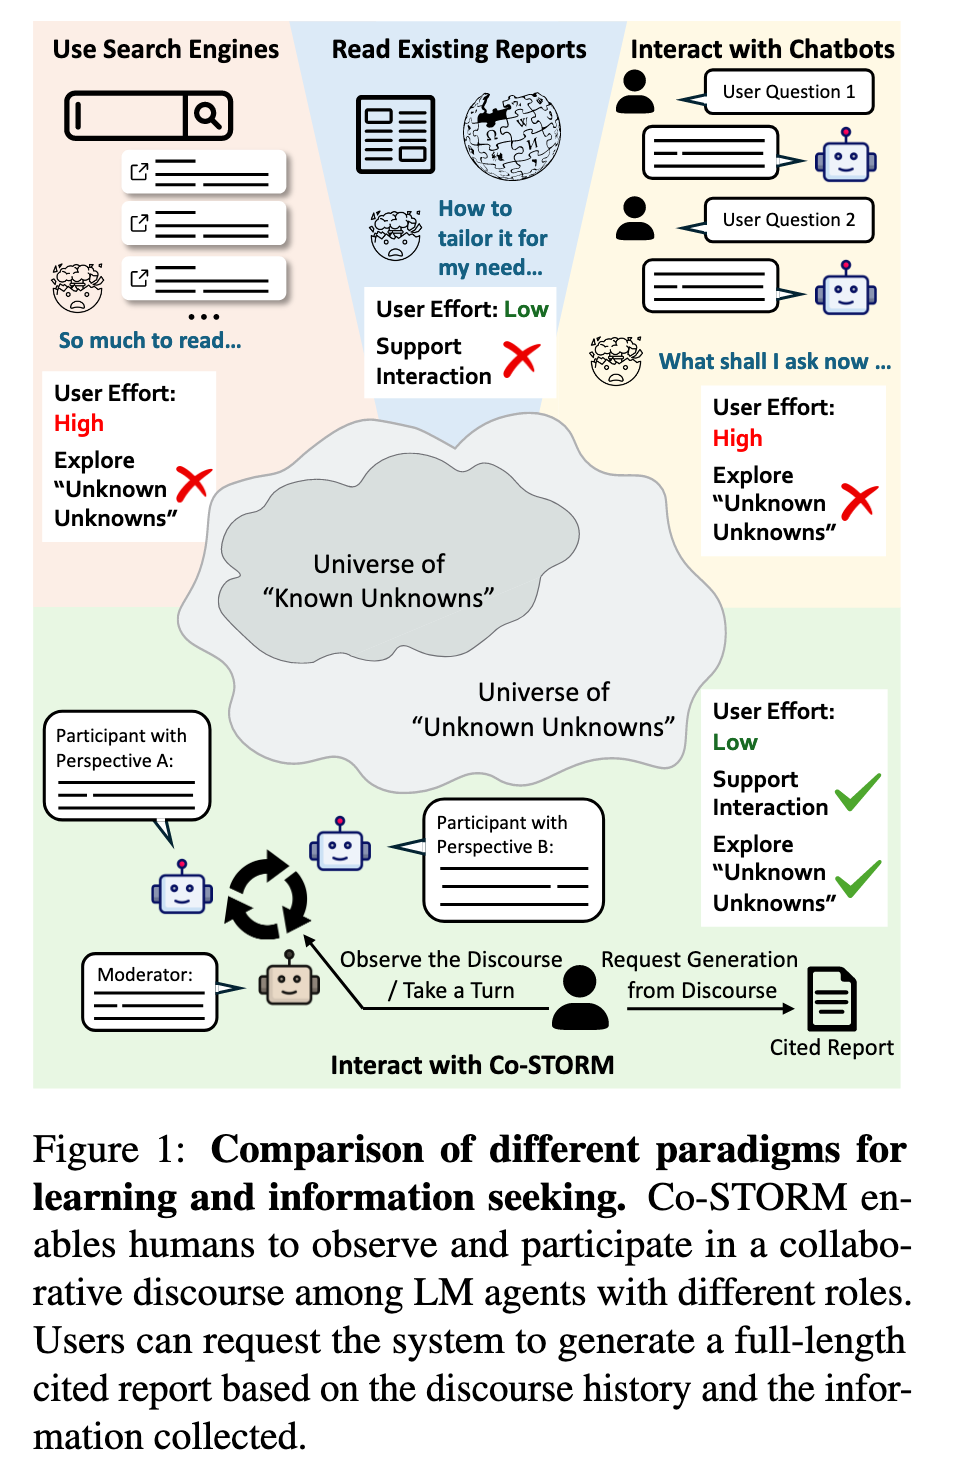
\includegraphics[width=5in,height=\textheight,keepaspectratio]{images/jiang_costorm_paradigms.png}

}

\caption{\label{fig-r-jiang-costorm}Diagram of the ``collaborative'' AI
discourse process which compares previous paradigms of information
seeking behavior based on user-effort, and their ability to explore
``unknown unknowns''. Taken from Jiang et al. (2024).}

\end{figure}%

The final piece of the policy-puzzle would be adding oversight
mechanisms that reinforce learning, accuracy, and ethical
interpretation. The ultimate goal being to promote dialectical learning
and information literacy (Doyle 1994): the question, response, and
knowledge integration process vital to promoting leadership skills in
the current, highly dynamic economy (Han, Bai, and Peng 2022). By seeing
the differing opinions of each AI agent instead of a singular response,
the required mediation of these different view-points inhibits analysts'
from over-relying on AI- a situation which leads to significantly worse
outcomes than humans and AI working separately (Passi and Vorvoreanu
2022).

\textbf{For senior staff}, policies should prioritize autonomous use-
ideally targeting the highly repetitive, low-effort/time-demanding
``back-of-house'' tasks like project management, file organization and
retrieval, and HR functions. Naturally, senior staff have significantly
higher standards for ensuring outputs align with institutional
objectives and legal boundaries, and thus a \emph{auditable} history of
AI actions is necessary before organizations can even begin considering
their adoption/integration ((PWC) Price Waterhouse Coopers n.d.).

Notably, the most accessible, popular AI tools (Gemini, ChatGPT,
Copilot) do \emph{not} inherently contain the oversight mechanisms
required for this policy to be implemented straight-away. In fact, for
the compliance/oversight function to be fulfilled, universities and
businesses must invest in the deliberate, contracted embedding of AI
models into the university's IT infrastructure similar to that of other
enterprise software (such as Google Workspace, or Zoom) such that its
queries and responses are auditable by the organization's compliance
departments. This contractual requirement is further elucidated below:

\subsubsection{AI Must Be Treated Like an Employee or
Consultant}\label{sec-r-governance}

AI systems employed in research commercialization workflows should be
governed under contractual clauses analogous to those applied to both
human consultants and staff, \emph{and} those of mission-critical
enterprise software. This includes documenting the scope of data privacy
for uploaded materials, (un)acceptable prompts for AI generated
material, and attributing the citation-source of relevant material in
all final deliverables.

According to the National Institute of Standards \& Technology's AI Risk
Management Framework (Tabassi 2023):

\begin{quote}
\emph{Third-party data or systems can accelerate research and
development and facilitate technology transition. They also may
complicate risk measurement. Risk can emerge both from third-party data,
software or hardware itself and how it is used. \textbf{Risk metrics or
methodologies used by the organization developing the AI system may not
align with the risk metrics or methodologies uses by the organization
deploying or operating the system.}}
\end{quote}

However, interactions with AI are via conversing with ``agents''- an
anthropomorphizing term which complicates contractual language for risk
mitigation. For example, third party AI providers may submit risk
metrics for their base-line LLM model, but not for the transformation of
that base-line LLM model into a role specific agent which the analysts
use as described in Section~\ref{sec-r-seniority}. Thus, risk mitigation
clauses for standard software/supplier relationships must be further
elucidated to encompass the potential risks of the AI ``agent/employee''
provided to the company.

Furthermore, the hiring company of that AI ``employee'' must have its
own internal performance governance structure- including periodic
performance evaluations, comparable to those used in team-performance
appraisals, wherein the employee and the system's collaborative
effectiveness are judged together. Such a policy reinforces
institutional \emph{and} individual responsibility, and
\emph{measurably} ensures the clustered topics of concerned outlined by
the literature review are not (un)wittingly enacted by university
stakeholders.

\section{Acknowledgements}\label{acknowledgements}

This research project would not have been possible without the extensive
support of the Georgetown Biotechnology Faculty: its Program Director,
Dr.~Ivica Labuda, and this course's instructor, Professor Khuyen Mai.

This project's mentor, Christon Hill, provided an incredible degree of
guidance, advocacy, and wisdom throughout this project; offering
opportunities to learn not only through the project itself, and also the
many thoughtful conversations along the way.

\section*{References}\label{references}
\addcontentsline{toc}{section}{References}

\phantomsection\label{refs}
\begin{CSLReferences}{1}{0}
\bibitem[\citeproctext]{ref-acs_growth_2012}
Acs, Zoltan J., David B. Audretsch, Pontus Braunerhjelm, and Bo
Carlsson. 2012. {``Growth and Entrepreneurship.''} \emph{Small Business
Economics} 39 (2): 289--300.
\url{https://doi.org/10.1007/s11187-010-9307-2}.

\bibitem[\citeproctext]{ref-aldridge_bayh-dole_2011}
Aldridge, T. Taylor, and David Audretsch. 2011. {``The Bayh-Dole Act and
Scientist Entrepreneurship.''} \emph{Research Policy} 40 (8): 1058--67.
\url{https://doi.org/10.1016/j.respol.2011.04.006}.

\bibitem[\citeproctext]{ref-noauthor_artificial_nodate}
{``Artificial Intelligence ({AI}) {\textbar} Nature Portfolio Editorial
Policies.''} n.d. Accessed April 16, 2025.
\url{https://www.nature.com/nature-portfolio/editorial-policies/ai}.

\bibitem[\citeproctext]{ref-doyle_information_1994}
Doyle, Christina S. 1994. {``Information Literacy in an Information
Society.''} \emph{{ERIC} Digest}, May.

\bibitem[\citeproctext]{ref-gottweis_towards_2025}
Gottweis, Juraj, Wei-Hung Weng, Alexander Daryin, Tao Tu, Anil Palepu,
Petar Sirkovic, Artiom Myaskovsky, et al. 2025. {``Towards an {AI}
Co-Scientist.''} \emph{Google {AI} Research}, February.

\bibitem[\citeproctext]{ref-gupta_chatgpt_2023}
Gupta, Maanak, Charankumar Akiri, Kshitiz Aryal, Eli Parker, and
Lopamudra Praharaj. 2023. {``From {ChatGPT} to {ThreatGPT}: Impact of
Generative {AI} in Cybersecurity and Privacy.''} \emph{{IEEE} Access}
11: 80218--45. \url{https://doi.org/10.1109/ACCESS.2023.3300381}.

\bibitem[\citeproctext]{ref-han_creating_2022}
Han, Guohong, Yuntao Bai, and Gang Peng. 2022. {``Creating Team
Ambidexterity: The Effects of Leader Dialectical Thinking and Collective
Team Identification.''} \emph{European Management Journal} 40 (2):
175--81. \url{https://doi.org/10.1016/j.emj.2021.06.004}.

\bibitem[\citeproctext]{ref-hoonakker_measuring_2011}
Hoonakker, Peter, Pascale Carayon, Ayse Gurses, Roger Brown, Kerry
McGuire, Adjhaporn Khunlertkit, and James M. Walker. 2011. {``Measuring
Workload of {ICU} Nurses with a Questionnaire Survey: The {NASA} Task
Load Index ({TLX}).''} \emph{{IIE} Transactions on Healthcare Systems
Engineering} 1 (2): 131--43.
\url{https://doi.org/10.1080/19488300.2011.609524}.

\bibitem[\citeproctext]{ref-hughes_reimagining_2025}
Hughes, Laurie, Tegwen Malik, Sandra Dettmer, Adil S. Al-Busaidi, and
Yogesh K. Dwivedi. 2025. {``Reimagining Higher Education: Navigating the
Challenges of Generative {AI} Adoption.''} \emph{Information Systems
Frontiers}, February. \url{https://doi.org/10.1007/s10796-025-10582-6}.

\bibitem[\citeproctext]{ref-noauthor_initiative_nodate}
{``Initiative on Pedagogical Uses of Artificial Intelligence. Georgetown
University - Center for New Designs in Learning \& Scholarship.''} n.d.
Accessed April 16, 2025. \url{https://ipai.georgetown.edu/}.

\bibitem[\citeproctext]{ref-jiang_into_2024}
Jiang, Yucheng, Yijia Shao, Dekun Ma, Sina J. Semnani, and Monica S.
Lam. 2024. {``Into the Unknown Unknowns: Engaged Human Learning Through
Participation in Language Model Agent Conversations.''} {arXiv}.
\url{https://doi.org/10.48550/arXiv.2408.15232}.

\bibitem[\citeproctext]{ref-joshi_likert_2015}
Joshi, Ankur, Saket Kale, Satish Chandel, and D. Pal. 2015. {``Likert
Scale: Explored and Explained.''} \emph{British Journal of Applied
Science \& Technology} 7 (4): 396--403.
\url{https://doi.org/10.9734/BJAST/2015/14975}.

\bibitem[\citeproctext]{ref-kim_discovering_2025}
Kim, Sang Yoon, Won Kyung Lee, Su Jung Jee, and So Young Sohn. 2025.
{``Discovering {AI} Adoption Patterns from Big Academic Graph Data.''}
\emph{Scientometrics} 130 (2): 809--31.
\url{https://doi.org/10.1007/s11192-024-05228-4}.

\bibitem[\citeproctext]{ref-noauthor_net_nodate}
{``Net Promoter Score ({NPS}): The Ultimate Guide. Qualtrics.''} n.d.
Accessed April 16, 2025.
\url{https://www.qualtrics.com/experience-management/customer/net-promoter-score/}.

\bibitem[\citeproctext]{ref-passi_overreliance_2022}
Passi, Samir, and Mihaela Vorvoreanu. 2022. {``Overreliance on {AI}
Literature Review.''} \emph{{AI} Ethics \& Effects in Engineering and
Research}.
\url{https://www.microsoft.com/en-us/research/wp-content/uploads/2022/06/Aether-Overreliance-on-AI-Review-Final-6.21.22.pdf}.

\bibitem[\citeproctext]{ref-penades_ai_2025}
Penadés, José R, Juraj Gottweis, Lingchen He, Jonasz B Patkowski,
Wei-Hung Weng, Tao Tu, Anil Palepu, Artiom Myaskovsky, and Annalisa
Pawlosky. 2025. {``{AI} Mirrors Experimental Science to Uncover a Novel
Mechanism of Gene Transfer Crucial to Bacterial Evolution,''} February.
\url{https://doi.org/10.1101/2025.02.19.639094}.

\bibitem[\citeproctext]{ref-pricewaterhousecoopers_managing_nodate}
(PWC) Price Waterhouse Coopers. n.d. {``Managing the Risks of Generative
{AI}. {PwC}.''} Accessed April 16, 2025.
\url{https://www.pwc.com/us/en/tech-effect/ai-analytics/managing-generative-ai-risks.html}.

\bibitem[\citeproctext]{ref-tabassi_artificial_2023}
Tabassi, Elham. 2023. {``Artificial Intelligence Risk Management
Framework ({AI} {RMF} 1.0).''} {NIST} {AI} 100-1. Gaithersburg, {MD}:
National Institute of Standards; Technology (U.S.).
\url{https://doi.org/10.6028/NIST.AI.100-1}.

\bibitem[\citeproctext]{ref-young_executive_2025}
Young, Todd, Michelle Rozo, Alex Padilla, Stephanie Bice, Ro Khanna,
Paul Arcangeli, Angela Belcher, et al. 2025. {``Executive Summary of
National Security Comission on Emerging Biotechnology 2025 Final
Report.''} United States Senate - National Security Comission.
\url{https://www.biotech.senate.gov/final-report/chapters/executive-summary/}.

\end{CSLReferences}




\end{document}
